% ------------------------------------------------------------------------
% ------------------------------------------------------------------------
% ICMC: Modelo de Trabalho Acadêmico (tese de doutorado, dissertação de
% mestrado e trabalhos monográficos em geral) em conformidade com 
% ABNT NBR 14724:2011: Informação e documentação - Trabalhos acadêmicos -
% Apresentação
% ------------------------------------------------------------------------
% ------------------------------------------------------------------------

% Opções: 
%   Qualificação         = qualificacao 
%   Curso                = doutorado/mestrado
%   Situação do trabalho = pre-defesa/pos-defesa (exceto para qualificação)
% -- opções do pacote babel --
% Idioma padrão = brazil
	%french,	    	% idioma adicional para hifenização
	%spanish,			% idioma adicional para hifenização
	%english,			% idioma adicional para hifenização
	%brazil				% o último idioma é o principal do documento
\documentclass[english,brazil]{packages/icmc}

% ---
% Pacotes Opcionais
% ---
\usepackage{rotating}           % Usado para rotacionar o texto
\usepackage[all,knot,arc,import,poly]{xy}   % Pacote para desenhos gráficos
% Este pacote pode conflitar com outros pacotes gráficos como o ``pictex''
% Então é necessário usar apenas um dos pacotes conflitantes
\usepackage{microtype}
\microtypesetup{nopatch=eqnum}

% ---
% Informações de dados para CAPA e FOLHA DE ROSTO
% ---
\titulo{Wireless Controller Area Network}
\autor[Cirillo, M.]{Matheus Henrique Dias Cirillo}
\orientador[Orientador:]{Prof. Dr.}{Adenilso da Silva Simão}
%\coorientador{Prof. Dr.}{Fulano de tal}
\curso{Computação}
\area{Sistemas Computacionais} % Área de concentração do trabalho
\data{10}{05}{2026} % Data do depósito
% ---


% ---
% RESUMOS
% ---

% Resumo em português
% conter no máximo 500 palavras
\textoresumo{
    Este trabalho apresenta o desenvolvimento e a avaliação em bancada do WCAN, uma ponte sem fio para integrar novos pontos de medição ao sistema de aquisição de dados de uma equipe de Fórmula SAE. A motivação é reduzir as limitações impostas pelo cabeamento em rodas, componentes aerodinâmicos e sensores externos ao veículo, preservando a semântica das mensagens CAN já usadas pela equipe. A solução foi implementada com ESP32, ESP-NOW, filas FreeRTOS, empacotamento de amostras, filtragem por identificador CAN e duas estratégias de transporte, broadcast e multicast. A campanha experimental utilizou cinco placas ESP32, frequências entre 10 Hz e 1000 Hz e diferentes topologias de sensores e receptores. Os resultados mostram que o broadcast com agrupamento de amostras manteve 100\% de entrega na suíte de referência, enquanto o multicast indicou potencial para múltiplos receptores, mas ainda apresentou limitações de descoberta e memória. Assim, o WCAN se mostra viável para aquisição sem fio em bancada, com validação embarcada ainda necessária.
    }{Fórmula SAE, Aquisição de dados, CAN, ESP-NOW, Comunicação sem fio}

% ---
% resumo em inglês
% ---
\textoresumo[english]{
    This work presents the development and bench evaluation of WCAN, a wireless bridge designed to add new measurement points to the data acquisition system of a Formula SAE team. The goal is to reduce wiring limitations on wheels, aerodynamic components and sensors placed outside the vehicle while preserving the CAN message semantics already used by the team. The solution was implemented with ESP32, ESP-NOW, FreeRTOS queues, sample batching, CAN identifier filtering and two transport strategies, broadcast and multicast. The experimental campaign used five ESP32 boards, transmission frequencies from 10 Hz to 1000 Hz and different sensor and receiver topologies. The results show that broadcast with sample batching achieved 100\% delivery in the baseline suite, while multicast showed potential for multiple receivers but still suffered from discovery and memory limitations. Therefore, WCAN is viable for bench wireless acquisition, although in-vehicle validation remains necessary.
    }{Formula SAE, Data acquisition, CAN, ESP-NOW, Wireless communication}
    
% ---
% Configurações de aparência do PDF final
% ---
% alterando o aspecto da cor azul
\definecolor{blue}{RGB}{41,5,195}

% informações do PDF
\makeatletter
\hypersetup{
		pdftitle={\@title}, 
		pdfauthor={\@author},
    	pdfsubject={Monografia final de conclusão de curso apresentada ao Instituto de Ciências Matemáticas e de Computação – ICMC-USP.},
	    pdfcreator={LaTeX with abnTeX2/ICMC-USP},
		pdfkeywords={\palavraschave}, 
		colorlinks=true,       		% false: boxed links; true: colored links
    	linkcolor=blue,          	% color of internal links
    	citecolor=blue,        		% color of links to bibliography
    	filecolor=magenta,      	% color of file links
		urlcolor=blue,
		bookmarksdepth=4
}
\makeatother
% --- 

% ----------------------------------------------------------
% ELEMENTOS PRÉ-TEXTUAIS
% ----------------------------------------------------------

% Inserir a ficha catalográfica
%\incluifichacatalografica{tex/pre-textual/fichaCatalografica.pdf}
%\incluifichacatalografica

% Inserir folha de aprovação
%\input{tex/folha-aprovacao}

% DEDICATÓRIA / AGRADECIMENTO / EPÍGRAFE
%\textodedicatoria*{tex/pre-textual/dedicatoria}
%\textoagradecimentos*{tex/pre-textual/agradecimentos}
%\textoepigrafe*{tex/pre-textual/epigrafe}

% Inclui a lista de figuras
%\incluilistadefiguras

% Inclui a lista de tabelas
\incluilistadetabelas

% Inclui a lista de quadros
%\incluilistadequadros

% Inclui a lista de algoritmos
%\incluilistadealgoritmos

% Inclui a lista de códigos
%\incluilistadecodigos

% Inclui a lista de siglas e abreviaturas
%\incluilistadesiglas

% Inclui a lista de símbolos
%\incluilistadesimbolos

% ----
% Início do documento
% ----
\begin{document}

% ----------------------------------------------------------
% ELEMENTOS TEXTUAIS
% ----------------------------------------------------------
\textual

\chapter{Introdução}
\label{chapter:introducao}
\section{Equipes de Fórmula SAE}
A Fórmula SAE é uma competição estudantil de âmbito mundial, organizada no Brasil
pela SAE Brasil e realizada anualmente \cite{sae_brasil_formula_sae}. As equipes são compostas por alunos
de engenharia de uma mesma universidade, que ao longo do ano projetam,
constroem e testam um protótipo de veículo monoposto de competição. Na edição
de 2025, a competição brasileira contou com 66 equipes inscritas, representando
64 instituições brasileiras de ensino superior de 11 estados e do Distrito
Federal, além de duas equipes do exterior \cite{sae_brasil_formula_sae_2025_inscritos}.

A competição é estruturada em provas estáticas e dinâmicas. As provas estáticas
avaliam o projeto de engenharia, o plano de negócios e o detalhamento de custos
e manufatura; as provas dinâmicas testam o desempenho do protótipo em situações
como aceleração, skidpad, autocross e endurance. A prova de endurance tem maior
peso na pontuação e exige que o veículo percorra aproximadamente 22 km sem
falhas \cite{fsaeonline_endurance_2026}. Dado o calendário anual, cada ciclo de
desenvolvimento é único: falhas nas provas representam a perda de um ano de
trabalho, o que impõe requisitos de robustez, confiabilidade e melhoria
contínua sobre todos os subsistemas do veículo.

Entre as equipes que participam da Fórmula SAE, a EESC-USP Formula SAE é o
caso estudado neste trabalho. Vinculada à Escola de Engenharia de São Carlos
(EESC) da Universidade de São Paulo (USP), a equipe reúne estudantes de vários
cursos para projetar, manufaturar e testar protótipos em competições nacionais
e internacionais \cite{eesc_usp_formula_sae_e22_2025}. Seu título mais recente foi
conquistado em 2025, quando venceu a categoria Combustão da 21ª Competição
Nacional de Fórmula SAE Brasil, garantindo vaga para a etapa mundial
\cite{eesc_usp_formula_sae_2025,sae_brasil_resultados_combustao_2025}.

Como equipe vencedora e de alto desempenho, a EESC-USP depende fortemente de
uma cadeia de suporte técnico que transforma dados experimentais em decisões
práticas. Esse vínculo entre a coleta de dados no carro e as intervenções no
projeto é o foco das próximas subseções.

\section{A Importância da Aquisição de Dados}
Em ambientes de competição automotiva, compreender o comportamento do veículo
é condição essencial para extrair seu máximo desempenho. Sensores distribuídos
ao longo do protótipo fornecem informações que permitem validar projetos de
engenharia, orientar ajustes de setup, monitorar a integridade dos sistemas
críticos em tempo real e comparar objetivamente o desempenho entre pilotos
\cite{schultz2017_formula_sae_telemetry,ashford2020_formula_sae_data_analysis}. Sem
instrumentação adequada, a equipe fica limitada ao feedback subjetivo dos
pilotos — valioso, mas muitas vezes insuficiente para decisões precisas.

A aquisição de dados converte observações qualitativas em grandezas
mensuráveis: pressão de freio, curso de suspensão, ângulo de esterço,
aceleração lateral, temperatura de óleo, entre outras. Esses sinais permitem
identificar trechos da pista onde o carro perde tempo, avaliar diferenças entre
pilotos e verificar se modificações realizadas entre sessões surtem o efeito
esperado. Assim, o sistema de aquisição funciona como o elo entre o trabalho
de bancada e as decisões tomadas em pista. Trabalhos acadêmicos mostram
diversas soluções de baixo custo para telemetria e aquisição em Fórmula SAE,
com combinações variadas de armazenamento local, comunicação sem fio e
visualização em tempo real \cite{stoffman2004_low_cost_racing_daq,visconti2019_formula_sae_telemetry,zanetti2013_formula_sae_wireless,lauro2021_formula_sae_telemetria}.

No caso da EESC-USP, o sistema de aquisição de dados foi consolidado ao longo de
vários anos de desenvolvimento e testes, em continuidade a trabalhos anteriores
de eletrônica embarcada para Fórmula SAE \cite{blatt2020_aquisicao_formula_sae}.

A arquitetura adotada baseia-se em dois módulos de aquisição com
microcontroladores STM32, interligados por um barramento CAN a 1 Mbit/s, que
também conecta outros módulos eletrônicos do veículo (controle, transmissor
e distribuição de energia), formando uma rede de nós de comunicação
coesa \cite{silva2009_rede_can_formula_sae}. Cada módulo lê sinais provenientes
de sensores analógicos e digitais instalados no carro — acelerômetro, giroscópio,
sensores de pressão de freio, potenciômetros de suspensão e de esterço, entre
outros — e os transmite periodicamente pela rede CAN.

Os dados são registrados localmente em cartão SD embarcado. Ao final de cada
sessão, os arquivos são extraídos e processados em um software dedicado, que
gera arquivos estruturados para análise em ferramentas especializadas. Esse
fluxo (registro embarcado + pós-processamento) permite à equipe acompanhar a
evolução do veículo e dos pilotos ao longo do ano, fornecendo uma base objetiva
para decisões de engenharia e planejamento de melhorias.



\chapter{O Problema}
\label{chapter:problema}
% Conteudo migrado de thesis/main.tex.
% O titulo do capitulo fica definido em thesis.tex.


\section{Limitações do Sistema Atual}

Embora o sistema de aquisição da equipe seja robusto e consolidado, sua arquitetura
cabeada impõe restrições estruturais que limitam a capacidade de instrumentação
do veículo. Essas limitações se manifestam em três cenários distintos, cada um
com suas próprias implicações práticas.

O primeiro cenário envolve componentes rotativos, como o interior das rodas.
Nesses pontos, a conexão com o chicote elétrico do veículo é tecnicamente
possível por meio de acopladores rotativos, porém a complexidade de instalação,
o custo e a fragilidade desses componentes em ambiente de competição tornam
a solução inviável na prática. Isso impede a leitura de sensores como temperatura
de cubo ou deformação de manga de eixo — informações de alto valor para a dinâmica
veicular.

O segundo cenário diz respeito a regiões onde o cabeamento interfere diretamente
no fenômeno a ser medido ou onde seu custo de instalação não se justifica pela
frequência de uso. A asa traseira é o exemplo mais crítico: trata-se de um componente
aerodinâmico cuja performance é sensível a qualquer perturbação no escoamento
de ar ao redor de sua superfície. Além disso, testes de instrumentação na asa
são pontuais e pouco frequentes, o que torna ainda menos justificável o
investimento em um chicote dedicado — tanto em termos de material quanto de
mão de obra para montagem e desmontagem a cada sessão.

O terceiro cenário extrapola os limites físicos do veículo. Sensores posicionados
fora do carro — como um sensor de passagem para detecção automática de voltas,
ou equipamentos de medição estacionários utilizados em testes controlados —
não têm como se comunicar com o sistema de aquisição embarcado por meios
cabeados. Essa limitação impede a integração de dados externos ao fluxo de aquisição,
obrigando a equipe a recorrer a registros manuais ou sistemas completamente
separados, sem sincronização temporal com os demais canais do carro.
% what are the limitations of our current setup
% where they are more proeminent



\chapter{Soluções Consideradas}
\label{chapter:solucoes-consideradas}
Diante das limitações identificadas, três abordagens foram consideradas para
expandir a capacidade de instrumentação do veículo, comparadas na Tabela~\ref{tab:solucoes-consideradas}.
A literatura sobre sensores sem fio em veículos destaca justamente a redução de
cabeamento, massa e custo de instalação como motivações recorrentes, embora a
confiabilidade do enlace passe a ser uma restrição central de projeto
\cite{tavares2008_wsn_automobiles,rahman2017_intravehicular_wsn,hashemi2014_intracar_multihop_wsn}.

\section{Cabeamento Dedicado}

A primeira opção consiste em aceitar os custos inerentes à arquitetura cabeada e investir na infraestrutura necessária para cada ponto de medição: acopladores rotativos para as rodas, chicotes dedicados para a asa traseira e extensões do chicote principal para outros pontos de difícil acesso. Essa abordagem preserva a arquitetura existente sem exigir nenhum desenvolvimento de \emph{software} ou \emph{hardware} adicional. No entanto, os custos associados a essa solução envolvem restrições financeiras e técnicas.

Do ponto de vista financeiro, a instrumentação de partes móveis rotativas requer acopladores rotativos (\emph{slip rings}) selados para mitigar ruídos elétricos decorrentes da rotação e resistir ao contato com água e poeira. Chicotes voltados ao ambiente veicular de competição costumam exigir conectores circulares selados e condutores com proteções térmicas e químicas adequadas \cite{blatt2020_aquisicao_formula_sae}, os quais possuem custos de aquisição superiores aos de cabos elétricos convencionais. Tecnicamente, embora a conexão física ofereça alta confiabilidade de sinal, o cabeamento físico e suas blindagens térmicas, blindagens eletromagnéticas e suportes mecânicos adicionam peso ao protótipo. Além disso, o direcionamento de fiação ao longo dos braços de suspensão expõe o chicote a esforços dinâmicos constantes. Há também a complexidade de projeto no roteamento tridimensional para evitar pontos de tração nos cabos durante o esterçamento, e a vulnerabilidade à fadiga mecânica dos condutores após ciclos contínuos de movimentação e vibração.

Além desses fatores, o cabeamento dedicado não viabiliza a aquisição de dados no terceiro cenário levantado (sensores externos ao veículo) e impõe limites ao reposicionamento ou expansão futura de sensores.

\section{Sistemas de Aquisição Independentes}

A segunda opção consiste em desenvolver módulos de aquisição autônomos, cada um com sua própria memória local para gravação dos dados. Esses módulos operariam de forma independente do sistema principal, sendo instalados nos pontos de interesse e recuperados após cada sessão de testes para extração dos dados. Para viabilizar a análise conjunta, seria necessário algum mecanismo de sincronização temporal entre os módulos e o sistema embarcado no carro.

Embora essa abordagem elimine a fiação de longa distância até o registrador central, ela desloca a questão de massa e volume físico para os próprios módulos. Cada unidade autônoma requer um invólucro de proteção contra impactos, circuitos de condicionamento de sinal, memória de armazenamento e uma bateria dedicada. A massa combinada desses componentes adiciona peso e volume localizado ao protótipo, o qual pode igualar ou até superar a massa de um chicote elétrico direto de curto comprimento. Adicionalmente, a solução introduz a complexidade de sincronização \emph{offline} (propensa a desvios temporais), a impossibilidade de acompanhar os dados em tempo real durante os testes e o risco de perda total de registros caso ocorra falha de alimentação ou avaria física no módulo.

\section{Solução Sem Fio}

A terceira opção, adotada neste projeto, é o desenvolvimento de uma ponte de comunicação sem fio entre os pontos de medição e o sistema de aquisição existente, conforme esquematizado na Figura~\ref{fig:wcan-semfio}. Nessa abordagem, um nó sensor captura os dados localmente e os transmite por rádio para um nó receptor conectado ao barramento CAN do veículo. O receptor injeta os dados na rede como se fossem provenientes de qualquer outro nó cabeado, tornando a comunicação sem fio transparente para o restante do sistema. Trabalhos de telemetria em Fórmula SAE mostram soluções semelhantes, integrando aquisição de dados e comunicação por rádio com a rede do veículo \cite{zanetti2013_formula_sae_wireless,visconti2019_formula_sae_telemetry,fernandes2022_formula_sae_wifi_can}.

\begin{figure}[htbp]
\centering
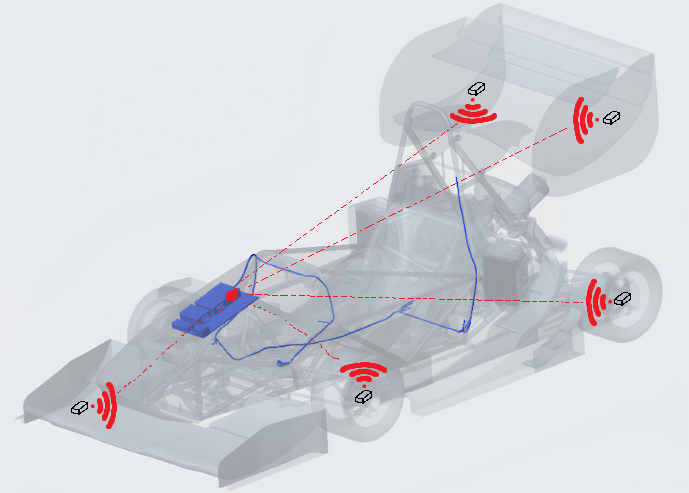
\includegraphics[width=0.85\textwidth]{images/wcan}
\caption{Arquitetura da solução sem fio proposta (WCAN) com transmissão via rádio para receptor central.}
\label{fig:wcan-semfio}
\end{figure}

Essa alternativa elimina a necessidade de roteamento de cabos de comunicação longos e acopladores rotativos, simplificando a instalação em componentes dinâmicos e externos ao carro. Contudo, assim como a aquisição independente, a ponte sem fio introduz peso localizado devido à necessidade de bateria, circuito de condicionamento, rádio e invólucro de proteção em cada nó sensor. Esse conjunto eletrônico pode apresentar massa superior à de uma conexão cabeada local direta de curto comprimento. Além disso, a comunicação sem fio adiciona o gerenciamento de recarga de baterias e o desafio técnico da confiabilidade do enlace, uma vez que a propagação de radiofrequência em ambientes veiculares está sujeita a atenuações e perda de pacotes, apresentando garantias de integridade inferiores às de uma conexão física metálica.

As vantagens e desvantagens de cada uma das alternativas consideradas para expandir a instrumentação estão sintetizadas na Tabela~\ref{tab:solucoes-consideradas}.

\begin{table}[htbp]
\centering
\small
\setlength{\tabcolsep}{4pt}
\renewcommand{\arraystretch}{1.18}
\begin{tabular}{p{0.22\linewidth}|p{0.34\linewidth}|p{0.34\linewidth}}
\hline
Solução & Vantagens & Desvantagens \\
\hline
Cabeamento dedicado &
Preserva a confiabilidade física do barramento CAN e exige baixo esforço de desenvolvimento de \emph{hardware}/\emph{software}. &
Adiciona fiação ao longo da estrutura do veículo; exige acopladores rotativos mecânicos em partes móveis; não atende a sensores externos. \\
\hline
Aquisição independente &
Elimina chicotes elétricos de longa distância; permite instalação em regiões de difícil acesso físico. &
Adiciona massa e volume localizado (bateria, circuitos e gabinete); exige sincronização \emph{offline}; impossibilita visualização em tempo real. \\
\hline
Ponte sem fio &
Remove fiação de longa distância; integra-se diretamente ao CAN existente; permite visualização de dados em tempo real. &
Adiciona massa e volume localizado (bateria, rádio e gabinete); exige desenvolvimento de protocolo de comunicação e tratamento de perda de pacotes. \\
\hline
\end{tabular}
\caption{Comparação das soluções consideradas para expandir a instrumentação do veículo.}
\label{tab:solucoes-consideradas}
\end{table}


\chapter{Requisitos}
\label{chapter:requisitos}
% Conteudo migrado de thesis/main.tex.
% O titulo do capitulo fica definido em thesis.tex.


Para que a solução sem fio seja viável em ambiente de competição, ela deve
satisfazer um conjunto de requisitos funcionais e não funcionais que
refletem tanto as restrições operacionais da equipe quanto as exigências
técnicas de integração com o sistema existente.

\section{Desempenho e Latência}

O sistema deve ser capaz de transmitir dados com latência compatível com as frequências
de aquisição já praticadas pela equipe. Atrasos na entrega dos dados
comprometem a sincronização temporal com os demais canais do sistema e podem
tornar a informação inutilizável para análise.

\section{Conexão Instantânea}

O sistema não pode depender de um processo de estabelecimento de conexão entre
os nós antes do início da transmissão. Em cenários como um sensor de
passagem externo ao veículo, o carro pode estar em alta velocidade quando passa
pelo ponto de medição — qualquer overhead de handshake inviabilizaria a coleta
do dado. A comunicação deve estar sempre pronta para transmitir, sem negociação
prévia entre os dispositivos.

\section{Múltiplas Conexões Simultâneas}

O sistema deve suportar múltiplos nós sensores transmitindo simultaneamente
para um ou mais receptores. Isso é especialmente relevante para a instrumentação
das quatro rodas do veículo, onde todos os sensores precisam operar em
paralelo e ter seus dados recebidos e injetados na rede CAN de forma
coordenada.

\section{Transparência com o Sistema CAN Existente}

A integração com o barramento CAN deve ser feita com o mínimo de modificações
possível na arquitetura existente. O sistema sem fio deve preservar os
identificadores CAN originais de cada mensagem e manter as verificações de
integridade nativas do protocolo — incluindo CRC e acknowledgment —
garantindo que o restante da rede trate os dados recebidos sem fio de forma
idêntica aos dados provenientes de nós cabeados.

\section{Requisitos Físicos e de Custo}

Os nós sensores devem ser fisicamente compactos e leves, uma vez que serão
instalados em regiões onde massa e volume são restrições relevantes — como
rodas e componentes aerodinâmicos. O custo total do sistema deve ser compatível
com o orçamento de uma equipe universitária, priorizando componentes
acessíveis sem comprometer os requisitos funcionais.

\section{Modularidade}

A arquitetura do sistema deve ser modular, permitindo adicionar novos nós
sensores sem alterações na infraestrutura existente. Cada novo ponto de medição
deve poder ser incorporado ao sistema de forma independente, com impacto
mínimo nos demais nós e sem necessidade de reconfiguração do receptor ou do
barramento CAN.
% what are the requirements for a successful system



\chapter{Framework}
\label{chapter:framework}
% Conteudo migrado de thesis/main.tex.
% O titulo do capitulo fica definido em thesis.tex.

\section{Microcontrolador}

A primeira decisão de hardware foi a escolha do microcontrolador para o nó sensor.
A opção mais natural inicialmente seria utilizar a família STM32, já presente
no sistema de aquisição da equipe e fornecida por um patrocinador. % TODO: confirmar patrocínio

A linha STM32 não possui nenhum chip com Wi-Fi nativo. A única família com comunicação
sem fio integrada é a STM32WB, que oferece Bluetooth Low Energy e 802.15.4 —
sem suporte a Wi-Fi. O STM32WB integra um núcleo Cortex-M4 para a aplicação
e um Cortex-M0+ dedicado ao stack de rádio, sendo uma plataforma robusta, bem
documentada e familiar à equipe \cite{st_stm32wb_series} — uma opção forte, desde que o BLE atendesse
aos requisitos de comunicação.

Para contornar a ausência de Wi-Fi nativo, uma alternativa seria combinar um
STM32 convencional com um módulo Wi-Fi externo. No entanto, essa abordagem exigiria
três componentes distintos na placa do nó sensor: o microcontrolador, o módulo
de comunicação e um circuito de gerenciamento de bateria separado. A
combinação resulta em uma solução com footprint físico, complexidade de integração
e custo de desenvolvimento incompatíveis com os requisitos de compacidade e leveza
do projeto, e foi descartada por esse motivo.

A terceira opção considerada foi o ESP32, plataforma da Espressif que integra
nativamente Wi-Fi e Bluetooth em um único chip. Módulos de desenvolvimento
compactos e com gerenciamento de bateria integrado estão amplamente
disponíveis para essa plataforma — como o Beetle ESP32-C3 da DFRobot, de
25×20,5 mm, que inclui gerenciamento de bateria na própria placa, sem
necessidade de componentes externos adicionais \cite{dfrobot_beetle_esp32c3}.

A decisão entre as duas plataformas foi tomada em conjunto com a escolha do protocolo
de comunicação, discutida a seguir.

% === SECTION: Protocolo de Comunicação Sem Fio ===

\section{Protocolo de Comunicação Sem Fio}

As opções naturais de protocolo para a solução sem fio foram Bluetooth Low Energy, Wi-Fi convencional e, posteriormente, ESP-NOW.

O BLE, disponível tanto no STM32WB quanto no ESP32, foi a primeira opção considerada. No entanto, o protocolo apresenta limitações importantes frente aos requisitos do sistema. O estabelecimento de uma conexão BLE envolve descoberta, pareamento ou associação entre dispositivos, o que introduz latência inicial e estado de conexão incompatíveis com a ideia de um sensor que pode começar a transmitir imediatamente. Além disso, o gerenciamento de múltiplas conexões simultâneas adicionaria complexidade significativa à aplicação. Essas limitações descartaram o BLE como protocolo principal e, por consequência, reduziram a atratividade do STM32WB para este projeto. Comparações experimentais entre ESP-NOW, Wi-Fi e Bluetooth também indicam que diferenças de latência, alcance e consumo tornam a escolha do protocolo dependente do perfil de aplicação \cite{eridani2021_espnow_wifi_bluetooth}.

O Wi-Fi convencional resolveria parte do problema de alcance e vazão, mas manteria o overhead de associação a uma rede, configuração de infraestrutura, obtenção de endereço IP e estabelecimento de sessão. Esse comportamento é inadequado para um sistema que deve funcionar sem ponto de acesso, sem configuração manual de rede e com início de transmissão o mais imediato possível.

Durante o desenvolvimento, foi adotado o ESP-NOW, protocolo proprietário da Espressif para comunicação direta entre dispositivos ESP32. O ESP-NOW opera sobre a camada física do Wi-Fi, mas não exige associação a uma rede Wi-Fi convencional. Os quadros são endereçados diretamente por endereço MAC, utilizam a verificação de integridade do próprio quadro 802.11, incluindo CRC em nível de enlace, e, na versão clássica utilizada neste trabalho, permitem até 250 bytes de payload por transmissão \cite{espressif_espnow_programming_guide,pasic2021_espnow_esp32}. Essa combinação atende aos requisitos de baixo overhead, operação sem infraestrutura e comunicação entre múltiplos dispositivos.

A principal limitação introduzida pelo ESP-NOW aparece no uso de broadcast. Quando um pacote é enviado para o endereço \texttt{FF:FF:FF:FF:FF:FF}, o transmissor não recebe uma confirmação nativa de entrega associada a cada receptor. Portanto, qualquer garantia de confiabilidade precisa ser construída acima do ESP-NOW, na camada de aplicação. Essa restrição motivou o desenvolvimento de duas variantes internas do transporte WCAN sobre o mesmo protocolo físico: uma variante broadcast, que preserva a semântica de barramento compartilhado do CAN, e uma variante unicast, que usa descoberta de receptores e confirmação do driver Wi-Fi por destinatário. As duas variantes implementam a mesma interface de aplicação e foram mantidas em paralelo para permitir comparação experimental em condições realistas, sem escolher antecipadamente uma solução definitiva.

Esse trade-off foi considerado aceitável porque o objetivo do projeto é expandir a aquisição de dados do veículo, não substituir por rádio uma malha de controle crítica. A camada WCAN pode acrescentar acknowledgments, retransmissões, filtragem, descoberta de receptores e medição de perdas, enquanto o ESP-NOW fornece a transmissão imediata e sem infraestrutura que os requisitos exigem. A escolha entre broadcast e unicast, portanto, deve ser guiada pelos resultados de entrega, latência e robustez observados nos ensaios, como também ocorre em outras soluções de telemetria veicular baseadas em Wi-Fi ou ESP32 \cite{fernandes2022_formula_sae_wifi_can}.


\chapter{Desenvolvimento}
\label{chapter:desenvolvimento}
A integração com o barramento CAN foi encapsulada em uma camada baseada no driver
TWAI da Espressif, que fornece a implementação de CAN clássico no ESP-IDF
\cite{espressif_twai_programming_guide}. Essa parte foi validada em bancada com
transceptores VP230, mas não foi o foco da campanha principal. Como a montagem em
protoboard introduzia falhas de contato, terminação e alimentação, os testes finais
isolaram a camada WCAN, que é a contribuição central deste trabalho.

\section{Arquitetura do WCAN}

O WCAN foi estruturado como um protocolo de aplicação sobre ESP-NOW. A interface
\texttt{wcan\_init} abstrai o transporte sem fio e permite que a aplicação trate os
dados recebidos como mensagens com semântica CAN. A camada empacota amostras por
identificador CAN, aplica filtros no receptor, envia os pacotes pelo rádio e entrega
os dados aceitos ao callback da aplicação.

Para suprir a necessidade de se investigar a viabilidade entre as abordagens citadas
anteriormente, foram implementadas duas variantes de transporte para o WCAN, broadcast 
e multicast, selecionadas em tempo de compilação. As duas usam o mesmo formato de pacote 
e a mesma aplicação de teste, o que permitiu comparar o impacto dessas estratégias de
endereçamento de forma isolada na confiabilidade sem alterar a instrumentação. O papel de 
cada placa, sensor, receptor ou nó ocioso, é definido no boot por uma linha enviada pela 
serial, junto com frequência de geração, CAN ID base, quantidade de IDs e valor de \texttt{linger\_ms}.

\section{Formato dos Pacotes}

A unidade de comunicação é a estrutura \texttt{data\_packet\_t}, composta pelo MAC
de origem, CAN ID, contador de ticks, quantidade de amostras e vetor de dados de 32
bits. Para transmissão, o pacote é serializado com 9 bytes de cabeçalho: 4 bytes de
CAN ID, 4 bytes de contador e 1 byte de quantidade de amostras. Como o ESP-NOW
clássico permite até 250 bytes de payload, restam 241 bytes para dados, o que limita
cada lote a 60 amostras de 4 bytes \cite{espressif_espnow_programming_guide}.

Os identificadores de controle foram colocados fora do espaço válido de IDs CAN
estendidos. Como o CAN estendido usa 29 bits, com valor máximo \texttt{0x1FFFFFFF},
a faixa \texttt{0xE0000000} foi reservada para sentinelas internas do WCAN
\cite{iso11898_1_2024}. No broadcast, esse valor identifica ACKs. No multicast,
identifica mensagens de descoberta, chamadas \texttt{HELLO}. Como apenas uma
variante é compilada por vez, não há conflito no firmware final.

\section{Filas e Agrupamento de Amostras}

Os callbacks do ESP-NOW foram mantidos curtos, conforme a recomendação da Espressif
de deslocar operações demoradas para filas e tasks de menor prioridade
\cite{espressif_espnow_programming_guide}. Na recepção, o callback apenas copia e
valida o pacote recebido. Filtragem, deduplicação, chamada da aplicação,
descoberta e retransmissões são tratadas fora desse contexto.

No caminho de transmissão, cada CAN ID possui uma fila própria. A task associada
consome amostras, espera até \texttt{linger\_ms} e fecha o lote quando a janela
expira ou quando 60 amostras são acumuladas. Esse batching é essencial porque o
ESP-NOW é um enlace de pacotes, com custo fixo por quadro. Para aquisição de dados
com frequência conhecida, o atraso controlado por \texttt{linger\_ms} reduz o uso do
canal e a pressão sobre filas. Quando \texttt{linger\_ms = 0}, o sistema envia uma
amostra por pacote, configuração mantida apenas como experimento de limite. Estudos
e medições práticas de ESP-NOW também indicam que tamanho de pacote, topologia e
condições do enlace afetam diretamente vazão e atraso \cite{hackaday_espnow_throughput,urazayev2023_indoor_espnow,wedyanti2025_espnow_multinode}.

\section{Transportes Broadcast e Multicast}

No broadcast, todos os pacotes de dados são enviados para
\texttt{FF:FF:FF:FF:FF:FF}. Os receptores no mesmo canal aplicam seus filtros por
CAN ID e, se aceitarem o pacote, enviam um ACK direcionado ao sensor. O transmissor
usa o par CAN ID e contador para correlacionar confirmações, retransmitindo quando
nenhum ACK válido chega dentro da janela esperada. Quando existem múltiplos
receptores, o primeiro ACK libera o próximo lote. Essa escolha replica a semântica
do ACK dominante do CAN, na qual o transmissor sabe que algum nó recebeu a
mensagem, mas não identifica quais nós a receberam \cite{iso11898_1_2024}.

No multicast, o sensor mantém uma tabela de assinantes interessados em cada CAN ID.
Enquanto não há assinantes vivos, o sensor transmite em broadcast para permitir
descoberta imediata. Um receptor interessado responde com \texttt{HELLO}, e o sensor
passa a incluí-lo nas próximas transmissões multicast. Receptores também enviam
\texttt{HELLO} periodicamente, permitindo que novos nós sejam descobertos mesmo após
o início da transmissão. O envio multicast usa o retorno do driver ESP-NOW como
sinal de sucesso no nível MAC, mas esse retorno não substitui uma confirmação
explícita de processamento pela aplicação \cite{espressif_espnow_programming_guide}.

As duas estratégias refletem compromissos diferentes. O broadcast é simples e
funciona sem descoberta prévia, mas só garante que ao menos um receptor interessado
confirmou o pacote. O multicast é o caminho natural para múltiplos receptores, mas
depende de descoberta, liveness e gerenciamento de memória mais robustos. Por isso,
a decisão entre as variantes foi tratada como questão experimental.

\section{Integração com o CAN Existente}

A integração preserva o CAN ID original. O receptor WCAN entrega um
\texttt{data\_packet\_t} à aplicação, que pode retransmitir os dados no barramento
físico via TWAI usando o mesmo identificador. Assim, os demais módulos do veículo
podem tratar os dados recebidos por rádio como mensagens CAN comuns
\cite{silva2009_rede_can_formula_sae,blatt2020_aquisicao_formula_sae}. Nos testes
quantitativos, o callback registrou os pacotes em log serial para análise de entrega
e latência. No uso embarcado, essa fronteira é o ponto de injeção no barramento CAN
local.


\chapter{Métodos}
\label{chapter:metodos}
Os ensaios foram planejados para avaliar a camada WCAN isoladamente, sem tornar
o barramento CAN físico o fator dominante da análise. A integração com TWAI foi
validada previamente em bancada com dois transceptores VP230, mas a campanha
principal concentrou-se no enlace sem fio, nas filas internas, na filtragem e nos
mecanismos de confirmação.

\section{Ambiente Experimental}

O ambiente experimental foi organizado em torno de um servidor Ubuntu usado como
ponto central de acesso remoto, orquestração e coleta dos testes. Essa escolha
facilitou o controle das placas espalhadas na bancada, a recuperação dos logs e a
execução dos scripts de automação sem depender de intervenção manual contínua.

A campanha utilizou cinco placas ESP32 conectadas por USB serial ao computador de
monitoramento, sendo três ESP32 e duas ESP32-C3. Em cada repetição, as placas
foram sorteadas como sensores, receptores ou nós ociosos, reduzindo a chance de
associar um resultado a uma placa específica. Cada ensaio durou 30 s, com três
repetições por topologia e 5 s de intervalo entre execuções.

O objetivo desse arranjo foi tornar a execução e a análise dos testes o mais
automáticas possível. Em vez de tratar cada ensaio como uma operação manual,
o ambiente foi estruturado para que a configuração, a sincronização dos papéis,
o registro das saídas e a posterior consolidação dos dados fossem conduzidos por
scripts.

\section{Automação dos Testes}

Os testes foram automatizados pelos scripts em \texttt{transmitter/testing}. O
arquivo \texttt{boards.yaml} descreve as placas disponíveis e o arquivo
\texttt{tests.yaml} define suítes, frequências, topologias, duração, repetições,
transporte, valor de \texttt{linger\_ms} e quantidade de CAN IDs por sensor. Antes
da execução, o runner gera \texttt{run\_plan.json} e, para cada teste, um
\texttt{scenario.json} com a topologia, os filtros e a linha de configuração
enviada a cada placa.

A \texttt{main.cpp} foi mantida como uma camada fina de inicialização e exemplo de
uso. Em vez de concentrar nela a lógica da automação de testes, o \texttt{app\_main} apenas
prepara o sistema, lê a configuração de boot e despacha a execução para módulos
específicos conforme o papel informado. A parametrização do ensaio fica isolada em
\texttt{runtime\_config.cpp}, enquanto o comportamento de sensor e receptor é
encapsulado, respectivamente, em \texttt{sensor\_app.hpp} e
\texttt{receiver\_app.hpp}. Essa separação permite reutilizar a mesma imagem de
firmware em diferentes papéis sem modificar o fluxo central, simplificando a
automação e a repetição dos testes.

Após gravar os firmwares necessários, o monitor serial reinicia as placas, aguarda
a mensagem \texttt{WCAN\_CFG\_WAIT} e envia por UART uma linha de configuração
específica para cada placa. Essa linha existe para que o firmware não precise ser
recompilado a cada repetição: ela informa o papel da placa, o transporte esperado, 
o CAN ID base do sensor, a quantidade de CAN IDs por sensor, a frequência de geração,
o valor de \texttt{linger\_ms} e, no caso de receptores, a lista de filtros de CAN ID. 
Em termos práticos, a mesma imagem de firmware pode atuar como sensor, receptor ou 
nó ocioso, e a distinção é feita apenas pelo conteúdo enviado nessa fase de boot. 
As saídas seriais são salvas separadamente por placa, o que permite reconstruir a 
sequência de eventos e inspecionar manualmente os casos reprovados.

\section{Matriz de Ensaios e Métricas}

A matriz principal de topologias incluiu todas as combinações com pelo menos um sensor e um 
receptor, limitadas pelo total de cinco placas disponíveis, isto é, \(S \geq 1\), \(R \geq 1\) 
e \(S + R \leq 5\). Isso resultou em dez topologias: 1S-1R, 1S-2R, 1S-3R, 1S-4R, 2S-1R, 2S-2R, 
2S-3R, 3S-1R, 3S-2R e 4S-1R.

A execução \texttt{full\_run} foi organizada em cinco suítes. A suíte \texttt{baseline} usou 
um CAN ID por sensor e \texttt{linger\_ms = 100}, servindo como referência de desempenho. 
A suíte \texttt{multiple} manteve \texttt{linger\_ms = 100}, mas configurou quatro CAN IDs por 
sensor, simulando um módulo de aquisição que publica vários sinais simultaneamente; nessa suíte 
também foi avaliada a variante multicast, adotada para múltiplos receptores interessados. A suíte 
\texttt{real\_time} configurou \texttt{linger\_ms = 0}, forçando cada amostra a ser enviada em 
seu próprio pacote ESP-NOW para medir o custo de operar sem batching. A suíte \texttt{active\_filter} 
usou pelo menos dois sensores e configurou allowlists nos receptores, validando a filtragem por 
CAN ID. Por fim, a suíte \texttt{mixed\_frequency} atribuiu frequências diferentes aos sensores 
de uma mesma topologia, sorteadas entre 100, 200, 750 e 1000 Hz, para verificar se fluxos rápidos 
prejudicam fluxos lentos.

\begin{table}[htbp]
\centering
\scriptsize
\setlength{\tabcolsep}{3pt}
\renewcommand{\arraystretch}{1.15}
\begin{tabular}{p{0.19\linewidth}|p{0.26\linewidth}|p{0.25\linewidth}|p{0.22\linewidth}}
\hline
Suíte & O que foi testado & Resultado esperado & Interpretação pretendida \\
\hline
\texttt{baseline} & Um CAN ID por sensor, \texttt{linger\_ms = 100}, varredura de 10 a 1000 Hz. & Entrega próxima de 100\% até frequências altas, pois o batching reduz a quantidade de pacotes. & Estabelecer a referência de desempenho do WCAN com batching. \\
\hline
\texttt{multiple} & Quatro CAN IDs por sensor, cada um com sua fila e sua task de processamento. & Aumentar a pressão sobre filas, timers e tarefas, mas sem colapsar se a arquitetura por CAN ID estiver correta. & Verificar concorrência entre fluxos do mesmo módulo. \\
\hline
\texttt{real\_time} & \texttt{linger\_ms = 0}, isto é, envio amostra a amostra. & Degradação em frequências altas, por aumento de overhead MAC e ocupação de filas. & Confirmar se batching é essencial para a proposta. \\
\hline
\texttt{active\_filter} & Receptores aceitando apenas subconjuntos dos CAN IDs transmitidos. & Receptores não devem entregar nem confirmar mensagens fora da allowlist. & Validar filtragem e comportamento de ACK com receptores parciais. \\
\hline
\texttt{mixed\_frequency} & Sensores na mesma topologia transmitindo em frequências diferentes. & Fluxos rápidos não devem impedir a entrega dos fluxos lentos. & Avaliar convivência entre sinais de naturezas diferentes. \\
\hline
\end{tabular}
\caption{Suítes executadas na campanha \texttt{full\_run} e objetivo de cada uma.}
\label{tab:suites-executadas}
\end{table}

\section{Métricas Coletadas}

A taxa de entrega foi calculada a partir dos valores de contador transportados pelos lotes. 
No lado sensor, o firmware registra uma linha \texttt{CAN\_PROC\_*} para cada lote colocado 
no transporte, contendo o CAN ID e o intervalo de contadores do lote, por exemplo \texttt{[0..59]}. 
No lado receptor, o callback \texttt{wcan\_recv\_callback} registra o mesmo intervalo quando 
o pacote é recebido. O script \texttt{analysis.py} reconstrói os intervalos recebidos e calcula 
a fração de contadores transmitidos que aparecem em pelo menos um receptor esperado. Na suíte 
de filtragem ativa, receptores cuja allowlist não contém determinado CAN ID não entram no 
denominador daquele fluxo.

Também foi analisada a entrega par a par entre cada sensor e cada receptor. Essa segunda métrica 
é informativa, mas não é o critério principal de sucesso do broadcast, porque o mecanismo de 
ACK dessa variante segue a semântica do CAN: se qualquer receptor interessado confirma o pacote, 
o transmissor considera a transmissão bem-sucedida. Portanto, um pacote pode ser aprovado na 
métrica principal e ainda assim não ter chegado a todos os receptores da topologia. Essa diferença 
é relevante para interpretar os resultados de topologias com múltiplos receptores.

A latência foi medida de formas diferentes nas estratégias de transporte, portanto os valores 
não devem ser comparados diretamente. No broadcast, a métrica \texttt{LAT\_RTT} registra o tempo 
de ida e volta, em milissegundos, até o recebimento do ACK de aplicação. No multicast, a métrica 
\texttt{LAT\_CB} registra, em microssegundos, o tempo entre a chamada a \texttt{esp\_now\_send()} 
e a execução do callback de transmissão do driver ESP-NOW. Esse segundo valor mede o retorno do driver 
e a confirmação no nível MAC, não a entrega fim a fim até o processamento da aplicação receptora.

O airtime foi estimado pela instrumentação do firmware. A cada janela periódica, o código acumula 
a quantidade de bytes transmitidos por ESP-NOW e, assumindo taxa física de 6 Mbps, estima a fração 
de tempo de canal consumida. O resultado é registrado nas linhas \texttt{MEASURE}, no campo 
\texttt{util\_per\_mille}, em partes por mil; 10 partes por mil correspondem a 1\% do tempo de canal. 
A estimativa ignora parte do overhead físico e deve ser interpretada como métrica relativa entre 
variantes.

Também foi coletado o high-water mark de pilha das tasks FreeRTOS. A instrumentação registra, nas 
linhas \texttt{TASK}, o campo \texttt{hwm\_bytes}, que indica o menor número de bytes livres observado 
na pilha daquela task. Valores abaixo de 100 bytes foram tratados como sinal de risco, pois indicam 
operação próxima de overflow de pilha. O analisador também verificou crashes, quedas de fila do 
produtor, quedas na fila interna do WCAN, falhas por limite de retry, lacunas em \texttt{RX\_STATS}, 
integridade de heap e validações específicas de cada suíte.


\chapter{Resultados dos Testes}
\label{chapter:resultados-testes}
\section{Visão Geral}

A campanha \texttt{full\_run} possuía 1116 execuções nominais. O analisador
consolidou 1115 pastas com logs suficientes e classificou 847 execuções como
aprovadas pelos critérios automáticos. A Tabela~\ref{tab:resumo-suites} resume os
resultados agregados mais relevantes.

\begin{table}[htbp]
\centering
\small
\setlength{\tabcolsep}{4pt}
\renewcommand{\arraystretch}{1.12}
\begin{tabular}{p{0.25\linewidth}|p{0.18\linewidth}|p{0.17\linewidth}|p{0.3\linewidth}}
\hline
Suíte e transporte & Aprovadas & Entrega & Leitura principal \\
\hline
\texttt{baseline}, broadcast & 150/150 & 100,00\% & Referência mais estável, sem perdas na métrica principal. \\
\hline
\texttt{multiple}, broadcast & 127/150 & 99,76\% & Suporta quatro IDs por sensor, mas expõe perdas pequenas. \\
\hline
\texttt{multiple}, multicast & 119/150 & 91,24\% & Promissor para múltiplos receptores, ainda frágil em descoberta e memória. \\
\hline
\texttt{real\_time}, broadcast & 56/149 & 91,77\% & Sem batching, filas e retries passam a limitar o sistema. \\
\hline
\texttt{active\_filter}, broadcast & 75/90 & 99,99\% & A filtragem funciona, mas a entrega par a par ainda varia. \\
\hline
\texttt{mixed\_frequency}, broadcast & 15/18 & 99,99\% & Frequências diferentes coexistem, com falhas ligadas sobretudo à geração local. \\
\hline
\end{tabular}
\caption{Resumo agregado das suítes executadas na campanha \texttt{full\_run}.}
\label{tab:resumo-suites}
\end{table}

O resultado central é que a variante broadcast com batching foi a única
configuração plenamente estável na matriz de referência. Com
\texttt{linger\_ms = 100}, a suíte \texttt{baseline} manteve 100\% de entrega em
todas as topologias e em frequências de 10 Hz a 1000 Hz. Foram analisados mais de
2,6 milhões de contadores sem perdas na métrica principal. A latência de
aplicação, medida por \texttt{LAT\_RTT}, ficou tipicamente em poucos
milissegundos, com mediana próxima de 3 ms entre 10 Hz e 200 Hz e próxima de
5 ms em 750 Hz e 1000 Hz.

\section{Efeito do Batching}

A suíte \texttt{real\_time} mostrou que o bom desempenho da linha de base depende
diretamente do agrupamento de amostras. Com \texttt{linger\_ms = 0}, cada amostra
é enviada em um quadro ESP-NOW independente. A entrega agregada do broadcast caiu
para 91,77\%, com 57970 quedas na fila do produtor e 231 falhas por limite de
retry. O sistema ainda se manteve quase estável em 10 Hz, mas perdeu robustez a
partir de 200 Hz e não teve execuções aprovadas em 1000 Hz.

Esse comportamento confirma que o WCAN não deve ser tratado como substituto sem
fio de uma rede CAN de controle em tempo real. Sua aplicação adequada é a
aquisição de dados com frequências conhecidas, na qual uma pequena janela de
agrupamento reduz o custo fixo de rádio, callbacks, filas e confirmações.

\section{Múltiplos Fluxos e Filtros}

Na suíte \texttt{multiple}, o broadcast manteve 99,76\% de entrega agregada mesmo
com quatro CAN IDs por sensor e mais de 4,3 milhões de contadores analisados. As
falhas apareceram como pequenas lacunas em receptores específicos ou como poucos
contadores ausentes em todos os receptores esperados. A primeira situação é
compatível com a semântica de primeiro ACK do broadcast, enquanto a segunda indica
perda efetiva, descarte em fila ou limite de retry.

A suíte \texttt{active\_filter} confirmou que receptores configurados com
allowlist não entregam nem confirmam mensagens fora de interesse. A entrega
agregada foi 99,99\%, mas apenas 75 de 90 execuções passaram por todos os
critérios. Em topologias com múltiplos receptores, um ACK válido prova que algum
receptor interessado recebeu o pacote, mas não que todos os receptores de interesse
receberam todos os contadores. Essa é uma limitação esperada do modelo adotado.

\section{Comportamento do Multicast}

O multicast foi avaliado principalmente na suíte \texttt{multiple}. A entrega
agregada de 91,24\% mostra que a estratégia é viável como direção de evolução,
mas ainda não está madura. Em casos representativos, sensores permaneceram por
muito tempo em modo de descoberta, registrando ausência de assinantes vivos mesmo
após receptores observarem pacotes iniciais. Sob carga, esse estado aumentou a
pressão sobre filas e heap, gerando erros como
\texttt{ESP\_ERR\_ESPNOW\_NO\_MEM} e, em alguns casos, reinicialização por falha
de alocação.

A investigação dos logs não apontou incompatibilidade de canal como causa
principal. O firmware fixa o canal ESP-NOW em 1 e não foram observados erros
característicos de canal incorreto. As falhas são melhor explicadas por
convergência incompleta de assinaturas, pressão de memória e falta de uma política
mais forte para períodos sem assinantes válidos.

\section{Limitações dos Ensaios}

Os resultados foram obtidos em bancada, com placas alimentadas e monitoradas por
USB. Essa configuração é adequada para comparar variantes e encontrar gargalos de
firmware, mas ainda não valida vibração, alimentação real, posicionamento de
antenas, interferência eletromagnética do carro, massa final do encapsulamento ou
injeção contínua no barramento CAN do veículo.

Também foram observados sinais de risco em memória e pilha. O menor high-water
mark de pilha observado nas agregações principais do broadcast foi 64 bytes, e os
logs multicast mostraram pressão de heap em períodos prolongados de descoberta.
Esses pontos não invalidam a linha de base, mas devem ser tratados antes de uma
validação embarcada prolongada.

\section{Rastreabilidade dos Requisitos}

A Tabela~\ref{tab:rastreabilidade-requisitos} resume o estado dos requisitos ao
final dos ensaios. O resultado mais forte é a validação em bancada do broadcast
com batching. Os requisitos ligados a múltiplos receptores, integração embarcada
e robustez física permanecem parciais.

\begin{table}[htbp]
\centering
\scriptsize
\setlength{\tabcolsep}{3pt}
\renewcommand{\arraystretch}{1.12}
\begin{tabular}{p{0.22\linewidth}|p{0.54\linewidth}|p{0.16\linewidth}}
\hline
Requisito & Evidência principal & Status \\
\hline
Desempenho e latência & Broadcast com batching entregou 100\% na suíte \texttt{baseline}, de 10 Hz a 1000 Hz. & Atendido em bancada \\
\hline
Conexão instantânea & Broadcast transmite sem associação prévia; multicast ainda falha quando a descoberta não converge. & Parcial \\
\hline
Múltiplas conexões & Topologias até cinco placas foram testadas; primeiro ACK não garante entrega a todos os receptores. & Parcial \\
\hline
Transparência CAN & O CAN ID é preservado e a fronteira de integração com TWAI foi definida, mas os testes finais usaram log serial. & Parcial \\
\hline
Requisitos físicos e custo & ESP32 reduz componentes e custo, mas placa final, fixação e massa ainda não foram validadas. & Parcial \\
\hline
Modularidade & Papéis por configuração serial, filtros por CAN ID e múltiplas frequências foram exercitados nos testes. & Atendido em bancada \\
\hline
\end{tabular}
\caption{Estado dos requisitos após a campanha de testes.}
\label{tab:rastreabilidade-requisitos}
\end{table}

\section{Conclusão dos Resultados}

Com os dados da campanha \texttt{full\_run}, a configuração mais defensável para
uso controlado é o broadcast com batching habilitado. Ela atende parcialmente ao
objetivo do trabalho ao permitir aquisição sem fio em bancada com semântica
próxima à do CAN, na qual uma mensagem é considerada confirmada quando algum
receptor interessado a reconhece. Para cenários em que todos os receptores devem
receber todos os pacotes, será necessário amadurecer o multicast ou introduzir
confirmação explícita por receptor.


\chapter{Conclusão}
\label{chapter:conclusao}
\section{Síntese do Trabalho}

Este trabalho apresentou o desenvolvimento e a avaliação experimental do WCAN, uma camada de comunicação sem fio baseada em ESP-NOW para transportar mensagens com semântica CAN entre módulos sensores e o sistema de aquisição de dados de um veículo de Fórmula SAE. A motivação principal foi reduzir a dependência de cabeamento em regiões de difícil instrumentação, como rodas, componentes aerodinâmicos e sensores externos ao veículo, sem exigir infraestrutura Wi-Fi, endereçamento IP ou mudanças profundas no modelo de dados já usado pela equipe.

A solução desenvolvida preserva o CAN ID como identificador lógico do sinal, agrupa amostras em pacotes ESP-NOW, usa filas FreeRTOS para desacoplar geração, transmissão e recepção, e inclui mecanismos de filtragem, confirmação e retransmissão. O trabalho também separou a camada WCAN da camada CAN física baseada no driver TWAI. Essa separação foi importante porque o driver CAN da Espressif já é uma base madura e validada, enquanto o ponto de incerteza deste projeto era a ponte sem fio. Os testes com transceptores VP230 em bancada indicaram que a integração CAN era funcional, mas a montagem em protoboard introduzia variabilidade suficiente para desviar a investigação do problema central. Por isso, a avaliação final concentrou-se no WCAN.

Os resultados da campanha \texttt{full\_run} mostram que o WCAN funciona bem em bancada quando usado no regime para o qual foi projetado: aquisição de dados com frequência conhecida, batching habilitado e tolerância a latências na ordem de milissegundos. A variante broadcast com \texttt{linger\_ms = 100} foi a configuração mais robusta. Ela manteve 100\% de entrega na suíte \texttt{baseline}, suportou múltiplas topologias de sensores e receptores e continuou operacional em frequências de até 1000 Hz na métrica principal de entrega.

O resultado mais importante da suíte \texttt{real\_time} foi mostrar que esse desempenho não vem simplesmente da taxa física do rádio. Sem batching, o sistema passa a ser limitado pela quantidade de pacotes ESP-NOW independentes, callbacks, filas, ACKs e retransmissões. Isso é coerente com o objetivo do projeto: o WCAN não pretende substituir uma rede CAN de controle em tempo real, mas expandir aquisição de dados em sensores amostrados com frequência conhecida. Nesse cenário, agrupar amostras por uma pequena janela de tempo é uma decisão aceitável e, pelos testes, necessária para operar em frequências altas.

A comparação entre variantes também deixa claro que a semântica de confiabilidade precisa ser escolhida de acordo com o uso. O broadcast é simples, robusto e adequado quando basta que ao menos um receptor interessado confirme o pacote, comportamento próximo à lógica de ACK dominante do CAN. Porém, essa semântica não garante que todos os receptores de uma topologia receberam todos os pacotes. Para esse requisito, a evolução natural é usar multicast com confirmação por assinante ou algum mecanismo equivalente de ACK por receptor.

\section{Problemas Conhecidos e Melhorias Futuras}

O principal problema conhecido da versão atual é o comportamento em situações sem assinantes válidos. Nos logs multicast, alguns sensores permaneceram tentando transmitir em modo de descoberta, mesmo quando nenhum assinante havia sido consolidado para aquele CAN ID. Em frequências altas, esse estado é perigoso: o sistema continua gerando pacotes, pressionando filas e heap, até registrar erros como \texttt{ESP\_ERR\_ESPNOW\_NO\_MEM} ou falhas de alocação dinâmica. Um sensor sem assinantes não deve derrubar a aplicação. O comportamento correto é tentar a descoberta por um número limitado de vezes, aplicar backoff, suspender temporariamente aquele fluxo ou descartar pacotes de forma controlada, registrar o evento e continuar executando.

Uma melhoria diretamente ligada a esse problema é reduzir alocações dinâmicas no caminho crítico de transmissão. A criação de pacotes por \texttt{new} ou \texttt{make\_unique} durante envio em alta frequência torna o sistema vulnerável a fragmentação, esgotamento de heap e falhas difíceis de reproduzir. Uma versão mais robusta deve usar buffers pré-alocados, pools de pacotes ou filas com capacidade fixa, de modo que o pior caso de memória seja conhecido antes da execução. Quando um pool estiver cheio, o sistema deve falhar de forma controlada, preferencialmente descartando a amostra mais nova ou mais antiga de acordo com a política definida, mas sem reiniciar a placa.

Também é necessário amadurecer a descoberta e a manutenção de assinantes. A transição entre broadcast de descoberta, registro de assinantes e envio multicast precisa ter estados explícitos, timeouts claros e métricas próprias. O \texttt{full\_run} mostrou que algumas falhas não eram perda de rádio em regime permanente, mas falhas de convergência: receptores podiam observar pacotes iniciais enquanto o transmissor não consolidava a tabela de assinantes. Uma melhoria futura é separar, nos logs e no protocolo, os eventos de descoberta, assinatura, expiração e reconexão, facilitando distinguir perda real de pacote de falha de controle.

Outra limitação é o dimensionamento de pilha e heap. O analisador encontrou high-water marks baixos em algumas tasks e, nos testes multicast, a ausência prolongada de assinantes válidos levou a pressão de memória suficiente para expor falhas de alocação. Mesmo quando esses casos não resultaram em crash, eles indicam pouca margem para uso embarcado prolongado. Antes de uma validação no veículo, é necessário revisar os tamanhos de stack, medir a ocupação por task em execuções longas, monitorar fragmentação de heap e transformar falhas de memória em erros recuperáveis.

A camada de análise também pode evoluir. A campanha \texttt{full\_run} evidenciou que uma repetição bem-sucedida não significa, sozinha, que a topologia é robusta, e uma repetição reprovada também não implica necessariamente falha sistemática do protocolo. O analisador já separa entrega, transporte, cenário, heap, crash e frequência observada, mas os resultados mostram a necessidade de classificar automaticamente falhas por causa provável: saturação, descoberta incompleta, receptor específico, ausência global de recepção, heap, pilha ou borda de teste. Isso tornaria a interpretação menos dependente de inspeção manual dos logs.

Do ponto de vista experimental, a próxima etapa é repetir as topologias críticas com mais repetições e duração maior. As suítes \texttt{mixed\_frequency} e algumas falhas isoladas do \texttt{baseline} apontam fragilidades, mas nem sempre têm repetições suficientes para separar variação experimental de erro sistemático. Testes longos também são importantes para validar se os alertas de heap são vazamentos reais, fragmentação acumulada ou apenas variação normal da execução.

Por fim, ainda falta a validação embarcada no veículo. A bancada é adequada para comparar variantes e encontrar gargalos de firmware, mas não reproduz vibração, alimentação real, posicionamento de antenas, interferência eletromagnética, massa final do encapsulamento e integração completa com o barramento CAN do carro. A partir dos resultados deste trabalho, a configuração mais indicada para essa etapa é broadcast com batching, seguida por uma nova rodada de multicast depois que o comportamento sem assinantes e o gerenciamento de memória forem corrigidos.

\section{Considerações Finais}

A contribuição principal deste trabalho foi demonstrar que uma ponte sem fio com semântica CAN é viável para aquisição de dados de Fórmula SAE quando seus limites são assumidos explicitamente. O WCAN não substitui o CAN físico em aplicações de controle crítico, mas pode reduzir cabeamento e permitir instrumentação modular em pontos onde a rede cabeada é difícil ou indesejável.

Os testes também foram úteis por mostrarem onde a solução ainda não está pronta. O broadcast com batching já é um candidato prático para uso controlado em bancada e futura validação no veículo. O multicast é conceitualmente o caminho certo para múltiplos receptores, mas precisa de uma política mais forte de descoberta, confirmação e memória. Com essas melhorias, o WCAN pode evoluir de protótipo funcional para uma camada de aquisição sem fio mais previsível, segura e integrada ao ecossistema de dados da equipe.



% ---
% Finaliza a parte no bookmark do PDF, para que se inicie o bookmark na raiz
% ---
\bookmarksetup{startatroot}% 
% ---

% ----------------------------------------------------------
% ELEMENTOS PÓS-TEXTUAIS
% ----------------------------------------------------------
\postextual

% ----------------------------------------------------------
% Referências bibliográficas
% ----------------------------------------------------------
\bibliography{references}

% ----------------------------------------------------------
% Apêndices
% ----------------------------------------------------------

% ---
% Inicia os apêndices
% ---
\begin{apendicesenv}

    \chapter{Artefatos da Campanha full\_run}
    \label{appendix:full-run}
    Este apêndice registra onde estão os dados usados para sustentar a análise
quantitativa do Capítulo~\ref{chapter:resultados-testes}. A campanha
\texttt{full\_run} corresponde à última rodada completa de testes executada com a
versão do firmware analisada nesta monografia. No repositório local, os artefatos
estão em \path{transmitter/testing/results/full_run}. A mesma campanha pode ser
consultada no
\href{https://github.com/cirillom/WCAN/tree/3b57f282a41413706ea0240b9030d72ff5438133/transmitter/testing/results/full_run}{repositório GitHub}.

A pasta contém o plano de execução, a configuração das placas, a configuração das
suítes, o resumo produzido pelo runner, o relatório consolidado do analisador e os
logs seriais de cada placa. Cada execução possui um \texttt{scenario.json} e um
conjunto de logs separados por papel e porta serial. Essa organização permite
recalcular as métricas agregadas e inspecionar manualmente casos reprovados.

Na matriz nominal, a campanha possuía 1116 execuções. O analisador consolidou 1115
pastas com logs suficientes e classificou 847 execuções como aprovadas. Como uma
reprovação pode envolver entrega, transporte, cenário, heap, crash ou frequência
observada, os resultados foram interpretados por classe de falha, não apenas pela
taxa bruta de aprovação.


\end{apendicesenv}
% ---


% ----------------------------------------------------------
% Anexos
% ----------------------------------------------------------

% ---
% Inicia os anexos
% ---
%\begin{anexosenv}
%
%    \chapter{Páginas Interessantes na Internet} 
%    \label{chapter:paginas-interessantes}
%    \input{tex/annex/paginas-interessantes}
%
%\end{anexosenv}
% ---

\end{document}
